\documentclass[9pt]{beamer}

%~~~~~~~~~~~~~~~~~~~~~~~~~~~~~~~~~~~~~~~~~~~~~~~~~~~~~~~~~~~~~~~~~~~~~~~~~~~~~~
% Code
\newcommand{\code}[1]{\textcolor{white!25!black}{\texttt{#1}}}
%~~~~~~~~~~~~~~~~~~~~~~~~~~~~~~~~~~~~~~~~~~~~~~~~~~~~~~~~~~~~~~~~~~~~~~~~~~~~~~

%~~~~~~~~~~~~~~~~~~~~~~~~~~~~~~~~~~~~~~~~~~~~~~~~~~~~~~~~~~~~~~~~~~~~~~~~~~~~~~
% Tikz
\usepackage{tkz-graph}
\usepackage{tikz}
\usetikzlibrary{arrows,automata}
\usepackage{tikz}
\usetikzlibrary{arrows,automata}
% def https://tex.stackexchange.com/questions/214400/tikz-dashes-and-closed-curves
\usetikzlibrary{decorations}

\tikzset{
  cycled dash pattern/.code args={on #1 off #2}{
    % Use csname so catcode of @ doesn't have do be changed.
    \csname tikz@addoption\endcsname{%
      \pgfgetpath\currentpath%
      \csname pgf@decorate@parsesoftpath\endcsname{\currentpath}{\currentpath}%
      % Length of path
      \pgfmathparse{\csname pgf@decorate@totalpathlength\endcsname}\let\lc=\pgfmathresult%
      % Length of pattern
      \pgfmathparse{#1+#2}\let\lp=\pgfmathresult%
      % Scaling factor for pattern
      \pgfmathparse{\lc/(\lp*round(\lc/\lp))}\let\f=\pgfmathresult%
      % Actually scale the pattern
      \pgfmathparse{#1*\f}\let\on=\pgfmathresult%
      \pgfmathparse{#2*\f}\let\off=\pgfmathresult%
      % Tell PGF to dash this line
      \pgfsetdash{{\on}{\off}}{0pt}}%
  }
}
% Def. Dr. César.
\usetikzlibrary{shapes,calc}
\tikzstyle{edge}=[shorten <=2pt, shorten >=2pt, >=stealth, line width=1.1pt]
\tikzstyle{edgeDottedR}=[shorten <=2pt, shorten >=2pt, >=stealth, line width=1.1pt, dashed, ->] %  dashed
\tikzstyle{edgeDottedL}=[shorten <=2pt, shorten >=2pt, >=stealth, line width=1.1pt, dashed, <-] %  dashed
\tikzstyle{edgeDotted}=[shorten <=2pt, shorten >=2pt, >=stealth, line width=1.1pt, dashed] %  dashed
\tikzstyle{edgeC}=[curve to, out=270,in=270,relative, dashed]
\tikzstyle{blueE}=[shorten <=2pt, shorten >=2pt, >=stealth, line width=1.5pt, blue]
\tikzstyle{redE}=[shorten <=2pt, shorten >=2pt, >=stealth, line width=1.5pt, red]
\tikzstyle{blackV}=[circle, fill=black, minimum size=6pt, inner sep=0pt, outer sep=0pt]
\tikzstyle{brownV}=[circle, fill=brown, draw, minimum size=6pt, line width=0.75pt, inner sep=0pt, outer sep=0pt]
\tikzstyle{brownE}=[shorten <=2pt, shorten >=2pt, >=stealth, line width=1.5pt, brown]
\tikzstyle{blueV}=[circle, fill=blue, draw, minimum size=6pt, line width=0.75pt, inner sep=0pt, outer sep=0pt]
\tikzstyle{redV}=[circle, fill=red, draw, minimum size=6pt, line width=0.75pt, inner sep=0pt, outer sep=0pt]
\tikzstyle{redSV}=[semicircle, fill=red, minimum size=3pt, inner sep=0pt, outer sep=0pt, rotate=225]
\tikzstyle{blueSV}=[semicircle, fill=blue, minimum size=3pt, inner sep=0pt, outer sep=0pt, rotate=225]
\tikzstyle{blackSV}=[semicircle, fill=black, minimum size=3pt, inner sep=0pt, outer sep=0pt, rotate=225]
\tikzstyle{vertex}=[circle, draw, minimum size=6pt, line width=0.75pt, inner sep=0pt, outer sep=0pt]
\tikzstyle{yellowV}=[circle, fill=yellow, draw, minimum size=6pt, line width=0.75pt, inner sep=0pt, outer sep=0pt]
\tikzstyle{greenV}=[circle, fill=green, draw, minimum size=6pt, line width=0.75pt, inner sep=0pt, outer sep=0pt]
%~~~~~~~~~~~~~~~~~~~~~~~~~~~~~~~~~~~~~~~~~~~~~~~~~~~~~~~~~~~~~~~~~~~~~~~~~~~~~~

%~~~~~~~~~~~~~~~~~~~~~~~~~~~~~~~~~~~~~~~~~~~~~~~~~~~~~~~~~~~~~~~~~~~~~~~~~~~~~~
% Include Figure
\usepackage{graphicx}
\usepackage{subcaption}
\usepackage{wrapfig}
%~~~~~~~~~~~~~~~~~~~~~~~~~~~~~~~~~~~~~~~~~~~~~~~~~~~~~~~~~~~~~~~~~~~~~~~~~~~~~~

%~~~~~~~~~~~~~~~~~~~~~~~~~~~~~~~~~~~~~~~~~~~~~~~~~~~~~~~~~~~~~~~~~~~~~~~~~~~~~~
% Use roboto Font (recommended)
\usepackage[sfdefault]{roboto}
\usepackage[utf8]{inputenc}
\usepackage[T1]{fontenc}
%~~~~~~~~~~~~~~~~~~~~~~~~~~~~~~~~~~~~~~~~~~~~~~~~~~~~~~~~~~~~~~~~~~~~~~~~~~~~~~

%~~~~~~~~~~~~~~~~~~~~~~~~~~~~~~~~~~~~~~~~~~~~~~~~~~~~~~~~~~~~~~~~~~~~~~~~~~~~~~
% Define where theme files are located. ('/styles')
\usepackage{styles/fluxmacros}
\usefolder{styles}
% Use Flux theme v0.1 beta
% Available style: asphalt, blue, red, green, gray
\usetheme[style=asphalt]{flux}
%~~~~~~~~~~~~~~~~~~~~~~~~~~~~~~~~~~~~~~~~~~~~~~~~~~~~~~~~~~~~~~~~~~~~~~~~~~~~~~

%~~~~~~~~~~~~~~~~~~~~~~~~~~~~~~~~~~~~~~~~~~~~~~~~~~~~~~~~~~~~~~~~~~~~~~~~~~~~~~
% Extra packages for the demo:
\usepackage{booktabs}
\usepackage{colortbl}
\usepackage{ragged2e}
\usepackage{schemabloc}
%~~~~~~~~~~~~~~~~~~~~~~~~~~~~~~~~~~~~~~~~~~~~~~~~~~~~~~~~~~~~~~~~~~~~~~~~~~~~~~
%~~~~~~~~~~~~~~~~~~~~~~~~~~~~~~~~~~~~~~~~~~~~~~~~~~~~~~~~~~~~~~~~~~~~~~~~~~~~~~
% Informations
\title{Análisis de Algoritmos II}
\subtitle{Un algoritmo de barrido de línea para agrupación espacial.\\
  \textbf{Profesores:}\\
  Jorge Urrutia Galicia\\
  Adriana Ramírez Vigueras\\
  Diego Jesús Favela Nava.}
\author{Aguilera Moreno Adrian.}
\institute{Facultad de Ciencias, UNAM}
\date{\today}
\titlegraphic{Imagenes/im1.png}
%~~~~~~~~~~~~~~~~~~~~~~~~~~~~~~~~~~~~~~~~~~~~~~~~~~~~~~~~~~~~~~~~~~~~~~~~~~~~~~

\begin{document}

% Generate title page
\titlepage

\begin{frame}
 \frametitle{Tabla de contenido.}
 \tableofcontents
\end{frame}
%\input{./Apartado01}
\section{Introducción.}
% Introducción
{\setbeamertemplate{background}{
\includegraphics[width=\the\paperwidth,height=\the\paperheight]{images/White.png}}
\begin{frame}
  \frametitle{Introducción}
  \framesubtitle{Problemas de visibilidad.} %%Subtítulo de la diapositiva (opcional)
  Determinar regiones de visibilidad de un objeto geométrico bajo restricciones es
  un problema muy estudiado en \textit{Geometría Computacional}.
  
  \centering \includegraphics[width=0.15 \paperwidth]{images/Visibility.png}
\end{frame}

\begin{frame}
  \frametitle{Introducción}
  \framesubtitle{Polígono de visibilidad.} %%Subtítulo de la diapositiva (opcional)
  Definimos un \underline{Polígono de visibilidad} como el polígono formado a partir
  de un punto $q$ dentro de un polígono dado, digamos $P$. Entonces, el polígono
  de visibilidad de $q$ definido como
  \[V(q) = \{p \in P\ \big|\ q \text{ visualiza a } p\}.\]
\end{frame}

\begin{frame}
  \centering \includegraphics[width=0.55 \paperwidth]{images/V(q)01.png}
\end{frame}

\begin{frame}
  \centering \includegraphics[width=0.55 \paperwidth]{images/V(q)02.png}
\end{frame}

\begin{frame}
  \centering \includegraphics[width=0.55 \paperwidth]{images/V(q)03.png}
\end{frame}

\begin{frame}
  \centering \includegraphics[width=0.55 \paperwidth]{images/V(q)04.png}
\end{frame}

\begin{frame}
  \centering \includegraphics[width=0.55 \paperwidth]{images/V(q)05.png}
\end{frame}

\begin{frame}
  \centering \includegraphics[width=0.55 \paperwidth]{images/V(q)06.png}
\end{frame}

\begin{frame}
  \centering \includegraphics[width=0.55 \paperwidth]{images/V(q)07.png}
\end{frame}

\begin{frame}
  \centering \includegraphics[width=0.55 \paperwidth]{images/V(q)08.png}
\end{frame}

\begin{frame}
  \centering \includegraphics[width=0.55 \paperwidth]{images/V(q)09.png}
\end{frame}

\begin{frame}
  \centering \includegraphics[width=0.55 \paperwidth]{images/V(q)10.png}
\end{frame}

\begin{frame}
  \centering \includegraphics[width=0.55 \paperwidth]{images/V(q)11.png}
\end{frame}

\begin{frame}
  \frametitle{Introducción}
  En partícular, podemos tener distintos tipos de polígonos.
  
  \begin{figure}
    \centering
    \includegraphics[width=0.75 \paperwidth]{./images/Casos.png}
    \caption*{Distintos casos para encontrar polígonos de visibilidad.}
  \end{figure}
  
  \textbf{Obs.} El polígono de visibilidad no, necesariamente, tiene que ser
  un polígono acotado.
\end{frame}


\subsection{Categorías.}
\input{./02CategoriasAgrupamientos}

\subsection{Alternativas.}
%%%%%%%%%%%%%%%%%%%%%%%%%%%%%%%% Introducción:
\begin{frame}[fragile]{Alternativas.}{}
  \begin{wrapfigure}{r}{0.25\textwidth} %this figure will be at the right
    \centering
    \includegraphics[width=0.25\textwidth]{./Imagenes/Aleatorios.png}
    \caption*{Aleatorios.}
  \end{wrapfigure}
  
  Algunas alternativas para agrupar son:
  \begin{enumerate}
  \item \textbf{Redes neuronales}.
  \item \textbf{k-means $+$ Algoritmos genéticos}.
  \item \textbf{Muestreos aleatorios}.
  \end{enumerate}

%  \begin{wrapfigure}{l}{0.25\textwidth}
%    \centering
%    \includegraphics[width=0.25\textwidth]{Imagenes/RedNeuronal.jpg}
%  \end{wrapfigure}
  \begin{justify}  
    Algunas alternativas para agrupar basadas en el entrenamiento inteligente,
    búsquedas aleatorias (como las heurísticas), y uso de algoritmos genéticos
    (como las colonias de hormigas) son recurridas cuando no podemos garantizar
    un ``buen'' agrupamiento.
  \end{justify}
  
  \begin{figure}
    \centering
    \begin{subfigure}[b]{0.3\textwidth}
      \includegraphics[width=\textwidth]{./Imagenes/RedNeuronal.jpg}
      \caption*{Redes Neuronales.}
    \end{subfigure}
    \begin{subfigure}[b]{0.3\textwidth}
      \includegraphics[width=\textwidth]{./Imagenes/Geneticos.jpeg}
      \caption*{K-means + Genéticos.}
    \end{subfigure}
  \end{figure}
\end{frame}


\subsection{Agrupación Espacial.}
%%%%%%%%%%%%%%%%%%%%%%%%%%%%%%%% Introducción:

\begin{frame}[fragile]{Agrupación Espacial:}{Propuestas I.}
  La agrupación espacial es un subconjunto espacial de agrupación. Este tipo
  de agrupamiento es relacionado, con frecuencia, a métodos gráficos.
  \begin{figure}
    \centering
    \begin{subfigure}[b]{0.3\textwidth}
      \includegraphics[width=\textwidth]{./Imagenes/LeyGeo.png}
      %\caption*{Redes Neuronales.}
    \end{subfigure}
    \begin{subfigure}[b]{0.2\textwidth}
      \includegraphics[width=\textwidth]{./Imagenes/Waldo_Tobler_2007.jpg}
      %\caption*{K-means + Genéticos.}
    \end{subfigure}
    \caption*{1era ley de la geografía.}
  \end{figure}
  \textbf{Propuestas:}
  \begin{itemize}
  \item Zahn sugiere trabajar con un gráfico completo (con vértices cada elemento en el espacio),
    construir el árbol de expansión mínima y eliminar los ``bordes'' más largos comparando las
    longitudes de los arcos con la longitud promedio, eliminando aquellos con longitud mayor al
    doble de la longitud promedio.
  \end{itemize}
\end{frame}

%%%%%%%%%%%%%%%%%%%%%%%%%%%%%%%% Introducción:

\begin{frame}[fragile]{Agrupación Espacial:}{Propuestas II.}
  \textbf{Propuestas:}
  \begin{itemize}
  \item Narendra sugiere el uso de diagramas de Voronoi para agrupar en
    tiempo $\mathcal{O}(n \log n)$. El problema de esta solución es que
    los algoritmos son dificiles de implementar.
  \item Kang usó triangulaciones de Delaunay y un diagrama dual de Voronoi.
    Después de construir la triangulación en $\mathcal{O}(n \log n)$, eliminamos
    las aristas con longitudes mayores a $d$.
  \item Yujian presentó un algoritmo de agrupamiento en subárboles máximos en
    distancia.
  \end{itemize}
  \textbf{¿Problemas? ...}
\end{frame}


\section{Algoritmo de agrupación espacial..}
\subsection{Ejecución.}
\input{./06Algoritmo}
\input{./07Algoritmo}
\input{./08Algoritmo}
%%%%%%%%%%%%%%%%%%%%%%%%%%%%%%%% Algoritmo: Iteración 3.

\begin{frame}[fragile]{Algoritmo:}{Iteración 3.}
  %%%%%%%%%%%%%%%%%%%%%%%%%%%%%%%%%%%%%%%%%%%%%%%%%%%%%%%%%%%%%%%%%%%%%%%%%% FIGURE 1
  \begin{figure}[ht!]
    \centering
    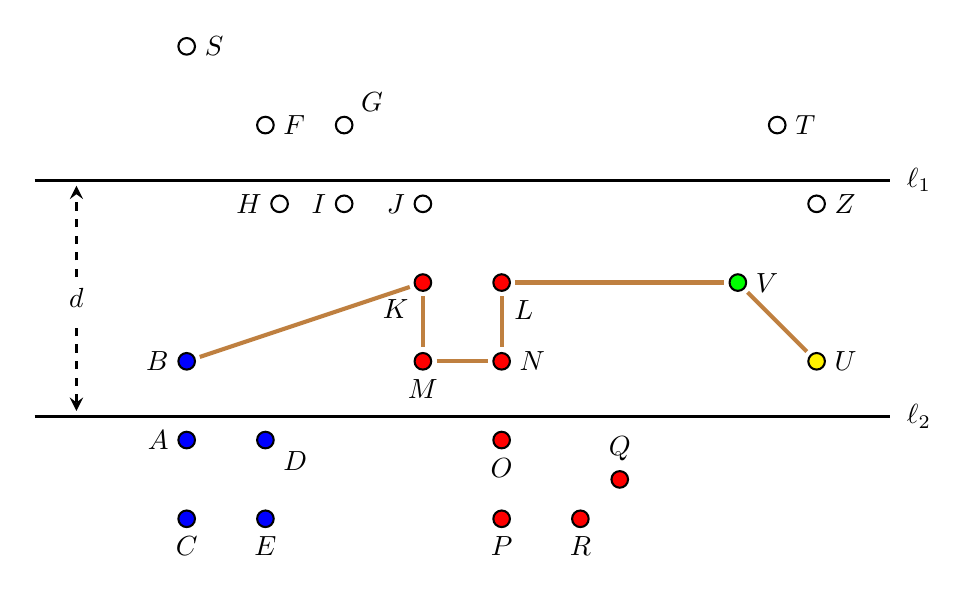
\begin{tikzpicture}
      %% Primer bloque:
      \node(A) [blueV, label=180:$A$] at (1, 5){};
      \node(B) [blueV, label=180:$B$] at (1, 6){};
      \node(C) [blueV, label=270:$C$] at (1, 4){};
      \node(D) [blueV, label=350:$D$] at (2, 5){};
      \node(E) [blueV, label=270:$E$] at (2, 4){};
      %% Segundo bloque:
      \node(S) [vertex, label=0:$S$] at (1,10){};
      \node(F) [vertex, label=0:$F$] at (2, 9){};
      \node(G) [vertex, label=30:$G$] at (3, 9){};
      \node(H) [vertex, label=180:$H$] at (2.18, 8){};
      \node(I) [vertex, label=180:$I$] at (3, 8){};
      \node(J) [vertex, label=180:$J$] at (4, 8){};
      \node(K) [redV, label=235:$K$] at (4, 7){};
      \node(L) [redV, label=290:$L$] at (5, 7){};
      \node(M) [redV, label=270:$M$] at (4, 6){};
      \node(N) [redV, label=000:$N$] at (5, 6){};
      \node(O) [redV, label=270:$O$] at (5, 5){};
      \node(P) [redV, label=270:$P$] at (5, 4){};
      \node(Q) [redV, label=90:$Q$] at (6.5, 4.5){};
      \node(R) [redV, label=270:$R$] at (6, 4){};
      %% Tercer bloque:
      \node(T) [vertex, label=0:$T$] at (8.5,9){};
      \node(Z) [vertex, label=0:$Z$] at (9,8){};
      \node(V) [greenV, label=0:$V$] at (8,7){};
      \node(U) [yellowV, label=0:$U$] at (9,6){};
      %% Rectas:
      \draw[edge] (-1,5.3) to (10,5.3); % l_2
      \draw[edge] (-1,8.3) to (10,8.3); % l_1
      % Distancia d:
      \draw[edgeDottedL] (-0.4,5.3) to (-0.4,6.5); % distancia abajo.
      \draw[edgeDottedR] (-0.4,7) to (-0.4,8.3);   % distancia arriba.
      % Nombres:
      \node (*) at (-0.4,6.8){$d$};
      \node (*) at (10.3,5.3){$\ell_2$};
      \node (*) at (10.3,8.3){$\ell_1$};
      
      % Frente de Avance:
      \draw[brownE] (B) to (K);
      \draw[brownE] (K) to (M);
      \draw[brownE] (M) to (N);
      \draw[brownE] (L) to (N);
      \draw[brownE] (L) to (V);
      \draw[brownE] (V) to (U);
      %\draw[brownE] (Q) to (U);
      % Proyecciones:
      %\node(PV) [blackV, label=270:$V'$] at (8, 5.4){};
      %\draw[edgeDotted] (V) to (PV);
      % Intento de círculo:
      %\draw[line with = 0.5pt, dash pattern = on 1pt off 2pt]circle(0.655cm);
      % The built-in version for comparison
      %\draw [line width=1pt, dash pattern=on 1pt off 2pt, black] (8,5.4) circle(1);
      %\draw [line width=1pt, dash pattern=on 1pt off 2pt, yellow] (9,6) circle(1);
      % Our version with automatically adapted pattern length
      %\draw [line width=1pt, cycled dash pattern=on 4pt off 4pt] (2,0) circle(0.655);
    \end{tikzpicture}
  \end{figure}
  %%%%%%%%%%%%%%%%%%%%%%%%%%%%%%%%%%%%%%%%%%%%%%%%%%%%%%%%%%%%%%%%%%%%%%%%%%
\end{frame}

\begin{frame}[fragile]{Algoritmo:}{Iteración 3.}
  %%%%%%%%%%%%%%%%%%%%%%%%%%%%%%%%%%%%%%%%%%%%%%%%%%%%%%%%%%%%%%%%%%%%%%%%%% FIGURE 1
  \begin{figure}[ht!]
    \centering
    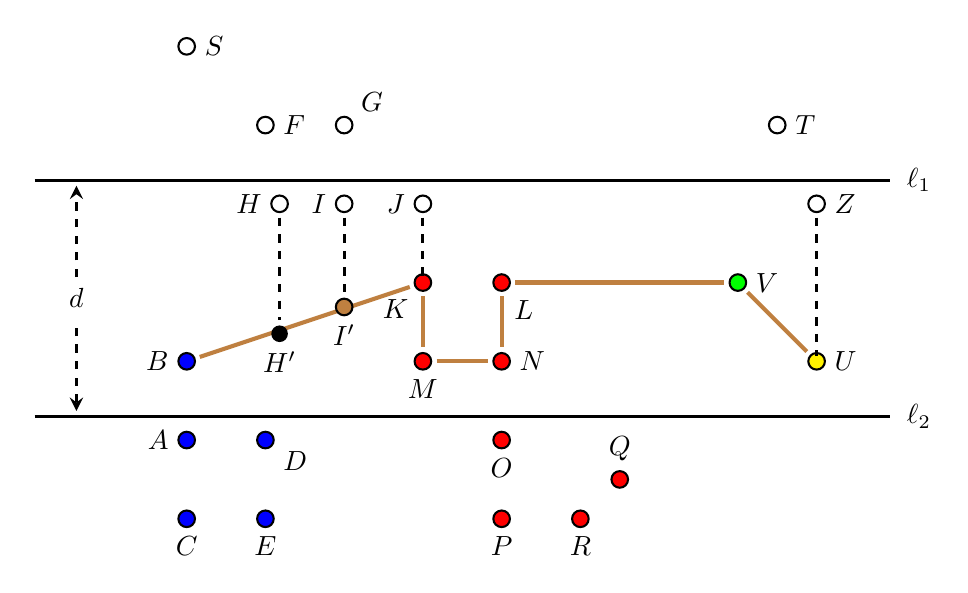
\begin{tikzpicture}
      %% Primer bloque:
      \node(A) [blueV, label=180:$A$] at (1, 5){};
      \node(B) [blueV, label=180:$B$] at (1, 6){};
      \node(C) [blueV, label=270:$C$] at (1, 4){};
      \node(D) [blueV, label=350:$D$] at (2, 5){};
      \node(E) [blueV, label=270:$E$] at (2, 4){};
      %% Segundo bloque:
      \node(S) [vertex, label=0:$S$] at (1,10){};
      \node(F) [vertex, label=0:$F$] at (2, 9){};
      \node(G) [vertex, label=30:$G$] at (3, 9){};
      \node(H) [vertex, label=180:$H$] at (2.18, 8){};
      \node(I) [vertex, label=180:$I$] at (3, 8){};
      \node(J) [vertex, label=180:$J$] at (4, 8){};
      \node(K) [redV, label=235:$K$]   at (4, 7){};
      \node(L) [redV, label=290:$L$] at (5, 7){};
      \node(M) [redV, label=270:$M$] at (4, 6){};
      \node(N) [redV, label=000:$N$] at (5, 6){};
      \node(O) [redV, label=270:$O$] at (5, 5){};
      \node(P) [redV, label=270:$P$] at (5, 4){};
      \node(Q) [redV, label=90:$Q$] at (6.5, 4.5){};
      \node(R) [redV, label=270:$R$] at (6, 4){};
      %% Tercer bloque:
      \node(T) [vertex, label=0:$T$] at (8.5,9){};
      \node(Z) [vertex, label=0:$Z$] at (9,8){};
      \node(V) [greenV, label=0:$V$] at (8,7){};
      \node(U) [yellowV, label=0:$U$] at (9,6){};
      %% Rectas:
      \draw[edge] (-1,5.3) to (10,5.3); % l_2
      \draw[edge] (-1,8.3) to (10,8.3); % l_1
      % Distancia d:
      \draw[edgeDottedL] (-0.4,5.3) to (-0.4,6.5); % distancia abajo.
      \draw[edgeDottedR] (-0.4,7) to (-0.4,8.3);   % distancia arriba.
      % Nombres:
      \node (*) at (-0.4,6.8){$d$};
      \node (*) at (10.3,5.3){$\ell_2$};
      \node (*) at (10.3,8.3){$\ell_1$};
      
      % Frente de Avance:
      \draw[brownE] (B) to (K);
      \draw[brownE] (K) to (M);
      \draw[brownE] (M) to (N);
      \draw[brownE] (L) to (N);
      \draw[brownE] (L) to (V);
      \draw[brownE] (V) to (U);
      %\draw[brownE] (Q) to (U);

      % Proyecciones:
      \node(PH) [blackV, label=270:$H'$] at (2.18, 6.35){};
      \draw[edgeDotted] (H) to (PH);
      \node(PI) [brownV, label=270:$I'$] at (3, 6.69){};
      \draw[edgeDotted] (I) to (PI);
      %\node(PJ) [blackV, label=270:$J'$] at (4, 7){};
      \draw[edgeDotted] (J) to (4,7);
      %\node(PZ) [blackV, label=270:$Z'$] at (9,6){};
      \draw[edgeDotted] (Z) to (9,6);

      % Intento de círculo:
      %\draw[line with = 0.5pt, dash pattern = on 1pt off 2pt]circle(0.655cm);
      % The built-in version for comparison
      %\draw [line width=1pt, dash pattern=on 1pt off 2pt, black] (2.18,6.35) circle(1);
      %\draw [line width=1pt, dash pattern=on 1pt off 2pt, brown] (PI) circle(1);
      % Our version with automatically adapted pattern length
      %\draw [line width=1pt, cycled dash pattern=on 4pt off 4pt] (2,0) circle(0.655);
    \end{tikzpicture}
  \end{figure}
  %%%%%%%%%%%%%%%%%%%%%%%%%%%%%%%%%%%%%%%%%%%%%%%%%%%%%%%%%%%%%%%%%%%%%%%%%%
\end{frame}

\begin{frame}[fragile]{Algoritmo:}{Iteración 3.}
  %%%%%%%%%%%%%%%%%%%%%%%%%%%%%%%%%%%%%%%%%%%%%%%%%%%%%%%%%%%%%%%%%%%%%%%%%% FIGURE 1
  \begin{figure}[ht!]
    \centering
    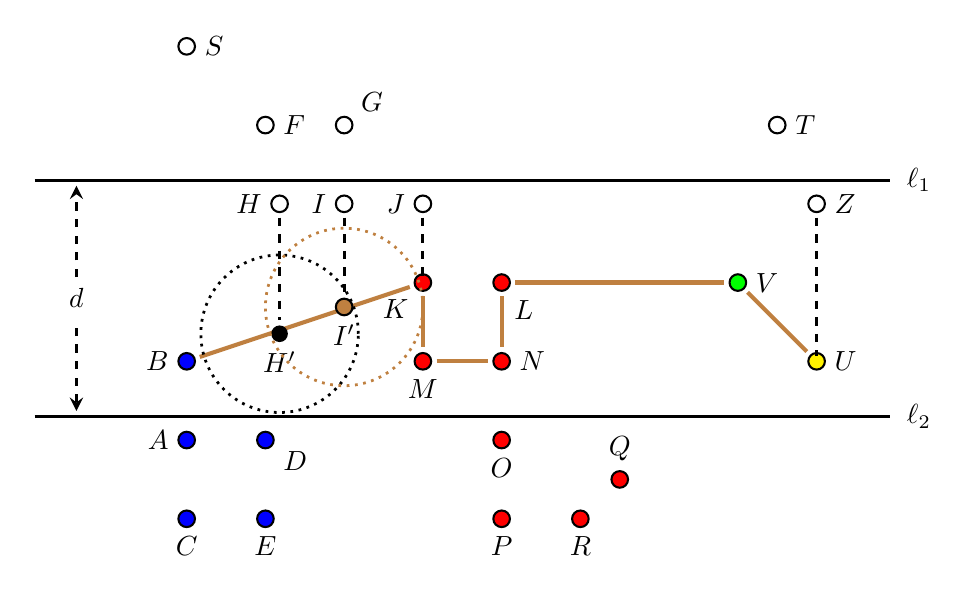
\begin{tikzpicture}
      %% Primer bloque:
      \node(A) [blueV, label=180:$A$] at (1, 5){};
      \node(B) [blueV, label=180:$B$] at (1, 6){};
      \node(C) [blueV, label=270:$C$] at (1, 4){};
      \node(D) [blueV, label=350:$D$] at (2, 5){};
      \node(E) [blueV, label=270:$E$] at (2, 4){};
      %% Segundo bloque:
      \node(S) [vertex, label=0:$S$] at (1,10){};
      \node(F) [vertex, label=0:$F$] at (2, 9){};
      \node(G) [vertex, label=30:$G$] at (3, 9){};
      \node(H) [vertex, label=180:$H$] at (2.18, 8){};
      \node(I) [vertex, label=180:$I$] at (3, 8){};
      \node(J) [vertex, label=180:$J$] at (4, 8){};
      \node(K) [redV, label=235:$K$]   at (4, 7){};
      \node(L) [redV, label=290:$L$] at (5, 7){};
      \node(M) [redV, label=270:$M$] at (4, 6){};
      \node(N) [redV, label=000:$N$] at (5, 6){};
      \node(O) [redV, label=270:$O$] at (5, 5){};
      \node(P) [redV, label=270:$P$] at (5, 4){};
      \node(Q) [redV, label=90:$Q$] at (6.5, 4.5){};
      \node(R) [redV, label=270:$R$] at (6, 4){};
      %% Tercer bloque:
      \node(T) [vertex, label=0:$T$] at (8.5,9){};
      \node(Z) [vertex, label=0:$Z$] at (9,8){};
      \node(V) [greenV, label=0:$V$] at (8,7){};
      \node(U) [yellowV, label=0:$U$] at (9,6){};
      %% Rectas:
      \draw[edge] (-1,5.3) to (10,5.3); % l_2
      \draw[edge] (-1,8.3) to (10,8.3); % l_1
      % Distancia d:
      \draw[edgeDottedL] (-0.4,5.3) to (-0.4,6.5); % distancia abajo.
      \draw[edgeDottedR] (-0.4,7) to (-0.4,8.3);   % distancia arriba.
      % Nombres:
      \node (*) at (-0.4,6.8){$d$};
      \node (*) at (10.3,5.3){$\ell_2$};
      \node (*) at (10.3,8.3){$\ell_1$};
      
      % Frente de Avance:
      \draw[brownE] (B) to (K);
      \draw[brownE] (K) to (M);
      \draw[brownE] (M) to (N);
      \draw[brownE] (L) to (N);
      \draw[brownE] (L) to (V);
      \draw[brownE] (V) to (U);
      %\draw[brownE] (Q) to (U);

      % Proyecciones:
      \node(PH) [blackV, label=270:$H'$] at (2.18, 6.35){};
      \draw[edgeDotted] (H) to (PH);
      \node(PI) [brownV, label=270:$I'$] at (3, 6.69){};
      \draw[edgeDotted] (I) to (PI);
      %\node(PJ) [blackV, label=270:$J'$] at (4, 7){};
      \draw[edgeDotted] (J) to (4,7);
      \draw[edgeDotted] (Z) to (9,6);
      
      % Intento de círculo:
      %\draw[line with = 0.5pt, dash pattern = on 1pt off 2pt]circle(0.655cm);
      % The built-in version for comparison
      \draw [line width=1pt, dash pattern=on 1pt off 2pt, black] (2.18,6.35) circle(1);
      \draw [line width=1pt, dash pattern=on 1pt off 2pt, brown] (PI) circle(1);
      % Our version with automatically adapted pattern length
      %\draw [line width=1pt, cycled dash pattern=on 4pt off 4pt] (2,0) circle(0.655);
    \end{tikzpicture}
  \end{figure}
  %%%%%%%%%%%%%%%%%%%%%%%%%%%%%%%%%%%%%%%%%%%%%%%%%%%%%%%%%%%%%%%%%%%%%%%%%%
\end{frame}

\begin{frame}[fragile]{Algoritmo:}{Iteración 3.}
  %%%%%%%%%%%%%%%%%%%%%%%%%%%%%%%%%%%%%%%%%%%%%%%%%%%%%%%%%%%%%%%%%%%%%%%%%% FIGURE 1
  \begin{figure}[ht!]
    \centering
    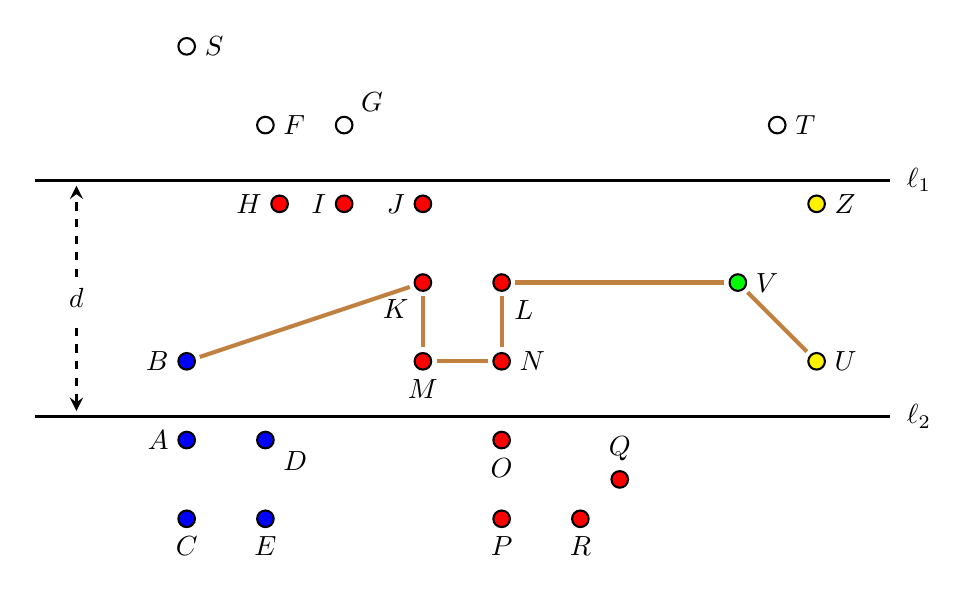
\begin{tikzpicture}
      %% Primer bloque:
      \node(A) [blueV, label=180:$A$] at (1, 5){};
      \node(B) [blueV, label=180:$B$] at (1, 6){};
      \node(C) [blueV, label=270:$C$] at (1, 4){};
      \node(D) [blueV, label=350:$D$] at (2, 5){};
      \node(E) [blueV, label=270:$E$] at (2, 4){};
      %% Segundo bloque:
      \node(S) [vertex, label=0:$S$] at (1,10){};
      \node(F) [vertex, label=0:$F$] at (2, 9){};
      \node(G) [vertex, label=30:$G$] at (3, 9){};
      \node(H) [redV, label=180:$H$] at (2.18, 8){};
      \node(I) [redV, label=180:$I$] at (3, 8){};
      \node(J) [redV, label=180:$J$] at (4, 8){};
      \node(K) [redV, label=235:$K$]   at (4, 7){};
      \node(L) [redV, label=290:$L$] at (5, 7){};
      \node(M) [redV, label=270:$M$] at (4, 6){};
      \node(N) [redV, label=000:$N$] at (5, 6){};
      \node(O) [redV, label=270:$O$] at (5, 5){};
      \node(P) [redV, label=270:$P$] at (5, 4){};
      \node(Q) [redV, label=90:$Q$] at (6.5, 4.5){};
      \node(R) [redV, label=270:$R$] at (6, 4){};
      %% Tercer bloque:
      \node(T) [vertex, label=0:$T$] at (8.5,9){};
      \node(Z) [yellowV, label=0:$Z$] at (9,8){};
      \node(V) [greenV, label=0:$V$] at (8,7){};
      \node(U) [yellowV, label=0:$U$] at (9,6){};
      %% Rectas:
      \draw[edge] (-1,5.3) to (10,5.3); % l_2
      \draw[edge] (-1,8.3) to (10,8.3); % l_1
      % Distancia d:
      \draw[edgeDottedL] (-0.4,5.3) to (-0.4,6.5); % distancia abajo.
      \draw[edgeDottedR] (-0.4,7) to (-0.4,8.3);   % distancia arriba.
      % Nombres:
      \node (*) at (-0.4,6.8){$d$};
      \node (*) at (10.3,5.3){$\ell_2$};
      \node (*) at (10.3,8.3){$\ell_1$};
      
      % Frente de Avance:
      \draw[brownE] (B) to (K);
      \draw[brownE] (K) to (M);
      \draw[brownE] (M) to (N);
      \draw[brownE] (L) to (N);
      \draw[brownE] (L) to (V);
      \draw[brownE] (V) to (U);
      %\draw[brownE] (Q) to (U);

      % Proyecciones:
      %\node(PH) [blackV, label=270:$H'$] at (2.18, 6.35){};
      %\draw[edgeDotted] (H) to (PH);
      %\node(PI) [brownV, label=270:$I'$] at (3, 6.69){};
      %\draw[edgeDotted] (I) to (PI);
      %\node(PJ) [blackV, label=270:$J'$] at (4, 7){};
      %\draw[edgeDotted] (J) to (4,7);
      %\draw[edgeDotted] (Z) to (9,6);
      
      % Intento de círculo:
      %\draw[line with = 0.5pt, dash pattern = on 1pt off 2pt]circle(0.655cm);
      % The built-in version for comparison
      %\draw [line width=1pt, dash pattern=on 1pt off 2pt, black] (2.18,6.35) circle(1);
      %\draw [line width=1pt, dash pattern=on 1pt off 2pt, brown] (PI) circle(1);
      % Our version with automatically adapted pattern length
      %\draw [line width=1pt, cycled dash pattern=on 4pt off 4pt] (2,0) circle(0.655);
    \end{tikzpicture}
  \end{figure}
  %%%%%%%%%%%%%%%%%%%%%%%%%%%%%%%%%%%%%%%%%%%%%%%%%%%%%%%%%%%%%%%%%%%%%%%%%%
\end{frame}

\input{./10Algoritmo}
\input{./11Algoritmo}
\subsection{Algoritmo.}
%%%%%%%%%%%%%%%%%%%%%%%%%%%%%%%% Algoritmo:

\begin{frame}[fragile]{Algoritmo:}{Especificación.}
  Nuestro algoritmo estara dividido en 3 fases:
  \begin{enumerate}
  \item \textbf{Inicialización}. Los puntos de entrada son ordenados
    con respecto a la dirección del movimiento de barrido.
  \item \textbf{Barrido}. Los grupos se construyen durante esta face, por medio
    de dos líneas de barrido $s_1$ y $s_2$.
  \item \textbf{Finalización}. Debemos unir los conglomerados.
  \end{enumerate}
\end{frame}

%%%%%%%%%%%%%%%%%%%%%%%%%%%%%%%% Algoritmo:

\begin{frame}[fragile]{Algoritmo:}{Barrido I.}
  \textbf{Barrido de línea.} Con $s_1$ y $s_2$ líneas, supongamos que estamos
  en la $i$-ésima iteración, entonces:
  \begin{enumerate}
  \item Los puntos entre ambas líneas de barrido se enlazan según sus coordenadas $X$,
    para formar una polilínea denominada FRENTE DE AVANCE (AF).
  \item Todos los puntos que han pasado por $s_1$ ya están contenidos en grupos $C_i$
    de acuerdo con el parámetro de proximidad $d$.
  \item Los puntos que han sido barridos por $s_2$ se eliminan de $AF$.
  \end{enumerate}
  \begin{figure}
    \centering
    \begin{subfigure}[b]{0.6\textwidth}
      \includegraphics[width=\textwidth]{./Imagenes/Barrido.png}
      \caption*{i-ésima iteración.}
    \end{subfigure}
  \end{figure}
\end{frame}

\begin{frame}[fragile]{Algoritmo:}{Barrido II.}
  \begin{figure}
    \centering
    \begin{subfigure}[b]{0.6\textwidth}
      \includegraphics[width=\textwidth]{./Imagenes/Barrido.png}
      \caption*{i-ésima iteración.}
    \end{subfigure}
  \end{figure}
  \begin{enumerate}
  \item[4.] En la siguiente iteración $s_1$ se mueve al siguiente punto y $s_2$ la sigue
    a distancia $d$.
  \item[5.] Cuando un punto $p_i$ ingresa a la manga entre las líneas $s_1$ y $s_2$, se determina
    su proyección con AF. Entonces puede pasar que:
    \begin{enumerate}
    \item[5.1] La proyección alcanza el AF.
    \item[5.2] La proyección no alcanza el AF.
    \end{enumerate}
    \textbf{Obs.} Diremos que $d_l = ||p_i - p_l||$ y $d_l = ||p_i - p_r||.$
  \end{enumerate}
\end{frame}

\begin{frame}[fragile]{Algoritmo:}{Barrido III.}
  \begin{figure}
    \centering
    \begin{subfigure}[b]{0.6\textwidth}
      \includegraphics[width=\textwidth]{./Imagenes/Barrido.png}
      \caption*{i-ésima iteración.}
    \end{subfigure}
  \end{figure}
  \begin{enumerate}
  \item[5.1] La proyección alcanza el AF. Entonces, sucede que
    \begin{enumerate}
    \item[5.1.1] Si $d_l > d$ y $d_r > d$. Entonces, $p_i$ forma un nuevo grupo.
    \item[5.1.2] Si $d_l \leq d$ y $dr > d$. Entonces, $p_i$ forma parte del grupo de $p_l$.
    \item[5.1.3] Si $d_l > d$ y $dr \leq d$. Entonces, $p_i$ forma parte del grupo de $p_r$.
    \item[5.1.4] Si $d_l \leq d$ y $dr \leq d$. Entonces, $p_r, p_l, p_i$ forman un grupo.
    \end{enumerate}
  \item[5.2] La proyección no alcanza el AF. Se compara contra el último más cercano en AF, si
    no pertenece a ningún grupo existente forma uno nuevo.
    
    \textbf{Obs.} Diremos que $d_l = ||p_i - p_l||$ y $d_l = ||p_i - p_r||.$
  \end{enumerate}
\end{frame}

%%%%%%%%%%%%%%%%%%%%%%%%%%%%%%%% Algoritmo:

\begin{frame}[fragile]{Algoritmo:}{Finalización.}
  Los índices conglomerador, que deben fusionarse se ajustan durante la fase de finalización.

  La estructura de datos, que almacena los índices de los grupos es una matriz de listas.
  \begin{figure}
    \centering
    \begin{subfigure}[b]{0.6\textwidth}
      \includegraphics[width=\textwidth]{./Imagenes/FusionConglomerados.png}
      \caption*{Estructura auxiliar.}
    \end{subfigure}
  \end{figure}
  En cada lista se conserva el registro que tiene el valor de índices más pequeño, mientras se eliminan.
\end{frame}

\subsection{Complejidad.}
%%%%%%%%%%%%%%%%%%%%%%%%%%%%%%%% Algoritmo:

\begin{frame}[fragile]{Algoritmo:}{Análisis de Complejidad.}
  \begin{enumerate}
  \item \textit{Inicialización.} Ordenar nuestro conjunto de puntos por comparaciones respecto
    al sentido de nuestro barrido nos toma $\mathcal{O}(n \log n)$.
  \item \textit{Barrido.} Al realizar una proyección para $p_i$ en AF debemos realizar una
    búsqueda en nuestro conjunto formado por AF (que hereda el orden de nuestro conjunto de puntos).
    Esto nos toma $\mathcal{O}(\log m)$ donde $m$ es el tamaño de AF. La complejidad total es $\mathcal{O}(n \log n)$.
  \item \textit{Finalización.} Fusionar los conglomerados se realiza en $c \cdot n \in \mathcal{O}(n).$
  \end{enumerate}
  
  \[\therefore \text{ La complejidad total del algoritmo esta contenida en } \mathcal{O}(n \log n).\]
\end{frame}

\subsection{Experimentación y resultados con grandes cantidades de datos.}
%%%%%%%%%%%%%%%%%%%%%%%%%%%%%%%% Experimentación:

\begin{frame}[fragile]{Experimentación:}{Experimento 1.}
  Para un conjunto de datos arbitrarios, nuestro algoritmo de
  agrupamiento reconoce grupos anidados en una forma arbitraria.
  \begin{figure}
    \centering
    \begin{subfigure}[b]{0.6\textwidth}
      \includegraphics[width=\textwidth]{./Imagenes/Exp1.png}
      \caption*{Agrupamiento anidado.}
    \end{subfigure}
  \end{figure}
  Conjunto con 753 puntos de datos obtenidos al trazar la imagen con
  MS Paint. $d$ fue establecida con respecto al $1\%$ del total de puntos.
  La cardinalidad se fijó en 1 y por consecuencia existen puntos aislados.
\end{frame}

%%%%%%%%%%%%%%%%%%%%%%%%%%%%%%%% Experimentación:

\begin{frame}[fragile]{Experimentación:}{Experimento 2.}
  Experimento realizado con $10,000$ puntos de información.
  \begin{figure}
    \centering
    \begin{subfigure}[b]{0.6\textwidth}
      \includegraphics[width=\textwidth]{./Imagenes/Exp2.png}
      \caption*{Agrupamiento con variación en $d$.}
    \end{subfigure}
  \end{figure}
  La cardinalidad de los grupos se fijo en 50 y se vario el parámetro $d$.
\end{frame}

% Fin
%%%%%%%%%%%%%%%%%%%%%%%%%%%%%%%% Fin:

\begin{frame}[fragile]{Fin.}{}
  \begin{figure}
    \centering
    \begin{subfigure}[b]{0.6\textwidth}
      \includegraphics[width=\textwidth]{./Imagenes/Agradecimientos.jpg}
      %\caption*{}
    \end{subfigure}
  \end{figure}
\end{frame}

%\def\beamer@mytheme@style{green}

%\subsection{Algoritmo.}
%\input{./04Definiciones} % Algoritmo.
%\input{./05Definiciones} % Propagación del tiempo vectorial.
%\input{./06Definiciones} % Propiedades.
%\input{./07Definiciones} % Reducción de costo en la comparación de dos vectores.
%\input{./08Definiciones} % Relación del tiempo vectorial y estados globales.

%\subsection{Desventajas.}
%\input{./09Desventajas}  % Desventajas.

% The [plain] causes the headlines, footlines, and sidebars
% to be suppressed. Useful for showing large pictures

% TODO. Sin implementar.
%\input{./Apartado02}
%\section{Aplicaciones.}
%\subsection{El caso DynamoDB.}
%\input{./Dynamo}
%\input{./Dynamo1}
%\input{./Dynamo2}
%\input{./Dynamo3}
%\input{./Dynamo4}
%\input{./Dynamo5}
%\input{./Dynamo6}
%\input{./Dynamo7}
%\input{./Dynamo8}
%\input{./Dynamo9}
%\input{./Dynamo10}
%\input{./Dynamo11}
%%%%%%%%%%%%%%%%% Nat:
% Solo es el orden, cambia lo que quieras (títulos). Perdón.
%----------------------------------------------------------
%\subsection{Relojes vectoriales dinámicos.}   %%%%%%%%%%%%%%%%%%%% Nat, aquí.  %%%%%%%%%%%%%%%%%%%%
%\input{./RVDinamicos01}
%\input{./RVDinamicos02}
%\input{./RVDinamicos03}
%\subsection{Seguimiento del predecesor inmediato (IPT).}
%\input{./IPT01}
%\input{./IPT02}
%\input{./IPT03}
%\input{./IPT04}
%\input{./IPT05}
%----------------------------------------------------------
%\subsection{Detección de una conjunción de predicados locales estables.}
%\input{./ConjunctionSatableLocalPredicates01}
%\input{./ConjunctionSatableLocalPredicates02}
%\subsection{Un problema de conjuntos: Conjuntos Posibles e Imposibles.}
%\input{./ProblemaConjuntos01}

%\input{./Apartado03}
%%%%%%%%%%%%%% Bloom: extra.
%\section{Relojes de Bloom.}
%\subsection{Filtro Bloom.}
%\input{./RelojesBloom01}
%\input{./RelojesBloom02}
%\input{./RelojesBloom03}
%\subsection{Algoritmo.}
%\input{./RelojesBloom04}
%\input{./RelojesBloom05}
%\input{./Agradecimientos}
\end{document}
